\documentclass[]{article}

\usepackage{amsmath}
\usepackage{amsfonts}
\usepackage{amssymb}
\usepackage{mathtools}
\usepackage{graphicx}
\usepackage{multirow}

\usepackage{multicol}


%opening
\title{}
\author{}

\begin{document}

\maketitle

\begin{abstract}

\end{abstract}


\newpage
%================================================================================%
%--------------------------------------------------------------------------------%
%================================================================================%
\section{The Hamiltonian of a charged particle in electromagnetic field}


The Lagrangian for a relativistic particle of mass $m$ with an electric charge $e$
in most general time-dependent electromagnetic field is given by
\[
	\mathcal{L}[\mathbf{r},\dot{\mathbf{r}};t] =
	-m\,c^2 \sqrt{1-\frac{\dot{\mathbf{r}}{}^2}{c^2}}
	-e\,\Phi(\mathbf{r},t)
	+e\left( \dot{\mathbf{r}} \cdot \mathbf{A}(\mathbf{r},t) \right),
\]
where $\mathbf{r}=(x,y,z)$ is a position vector of a particle in three dimensional
right handed Cartesian coordinate system
$\{\hat{\mathbf{e}}_x,\hat{\mathbf{e}}_y,\hat{\mathbf{e}}_z\}$
and $\dot{\mathbf{r}}=(\dot{x},\dot{y},\dot{z})$ being matching generalized
velocities, the action of dot differential operator is the derivative with respect to time $\dot{(\ldots)}\equiv\frac{\mathrm{d}}{\mathrm{d}t}$,
$\Phi(\mathbf{r},t)$ and $\mathbf{A}(\mathbf{r},t)$ are the electric scalar and
magnetic vector potentials respectively, and, $c$ is the speed of light in vacuum.

The Hamiltonian is constructed using the Legendre transformation of
$\mathcal{L}$
\[
	\mathcal{H} = \sum_{q=\{x,y,z\}} \dot{q}\, p_q - \mathcal{L},
\]
where $p_q$ are components of the particle's canonical momentum
\[
	\mathbf{p} \equiv \frac{\partial\,\mathcal{L}}{\partial\,\dot{\mathbf{r}}} =
		\frac{ m\,\dot{\mathbf{r}} }
			 { \sqrt{1-\frac{\dot{\mathbf{r}}^2}{c^2}} } +
		e\,\mathbf{A}(\mathbf{r},t),
\]
which gives
\[
	\mathcal{H}[\mathbf{p},\mathbf{q};t] =
	c \sqrt{ m^2c^2 + \left( \mathbf{p}-e\,\mathbf{A}(\mathbf{r},t) \right)^2 }
	+e\,\Phi(\mathbf{r},t).
\]

\newpage
%================================================================================%
%--------------------------------------------------------------------------------%
%================================================================================%
\section{R-elements}

\newpage
%================================================================================%
%--------------------------------------------------------------------------------%
%================================================================================%
\subsection{Electrostatic Lenses}

\[
	\mathcal{H}[p_x,p_y,p_s;x,y,s;t] =
	c \sqrt{ m^2c^2 + \mathbf{p}^2 }
	+e\,\Phi(x,y).
\]

\newpage
%================================================================================%
%--------------------------------------------------------------------------------%
%================================================================================%
\subsection{Magnetostatic Lenses}

\[
	\mathcal{H}[p_x,p_y,p_s;x,y,s;t] =
	c \sqrt{ m^2c^2 + p_x^2 + p_y^2 +
		\left( p_s - e\,A_s(x,y) \right)^2 }.
\]

%--------------------------------------------------------------------------------%
Introducing an extended Hamiltonian with a new time parameter, $\tau$, where the old independent variable and old Hamiltonian with a negative sign will be treated
as an additional pair of canonically conjugated coordinates, $(-\mathcal{H},t)$,
one have:
\[
\mathcal{O} [p_x,p_y,p_s,-\mathcal{H};x,y,s,t;\tau] \equiv 0 =
	c \sqrt{ m^2c^2 + p_x^2 + p_y^2 + \left( p_s - e\,A_s(x,y) \right)^2 } -
	\mathcal{H}.
\]
Integration of additional equations of motion gives
\begin{align}
\frac{\partial\,\mathcal{O}}{\partial t}\,\,\,\,		&= -
\frac{\mathrm{d}(-\mathcal{H})}{\mathrm{d}\tau},
	&\rightarrow&
& \mathcal{H} &= \mathrm{inv},												\\
\frac{\partial\,\mathcal{O}}{\partial(-\mathcal{H})}	&= \quad\,\,\,\,
\frac{\mathrm{d}\,t}{\mathrm{d}\tau},
	&\rightarrow&
& t &= \tau + C_0,
\end{align}
where we can set a constant of integration $C_0=0$.

%--------------------------------------------------------------------------------%
As a next step we will use longitudinal coordinate, $s$, as an independent
variable and $-p_s$ as a new Hamiltonian, reducing number of degrees of freedom
back up to three:
\[
	\mathcal{K}[p_x,p_y,-\mathcal{H};x,y,t;s] \equiv -p_s =
	- \sqrt{ \left(\frac{\mathcal{H}}{c}\right)^2 - m^2c^2 - p_x^2 - p_y^2}
	- e\,A_s(x,y).
\]
The use of generating function
\[
	G_2(t,-p) = - t \sqrt{p^2c^2+(m\,c^2)^2}
\]
will allow to use the full momentum $-p$ of a particle instead of $-\mathcal{H}$
as one of canonical momentums:
\[
	\mathcal{K}[p_x,p_y,-p;x,y,l;s] \equiv -p_s =
	- \sqrt{ p^2 - p_x^2 - p_y^2}
	- e\,A_s(x,y),
\]
where corresponding canonical coordinate is a particle's traversed path
\[
	l = \frac{\partial\,G_2(t,-p)}{\partial(-p)} = \beta c\,t.
\]

%--------------------------------------------------------------------------------%
Since the Hamiltonian do not explicitly depends on $l$, full momentum $p$ is
conserved and we can exclude associated degree of freedom using the further
renormalization of the Hamiltonian $\mathcal{K} \rightarrow K \equiv \mathcal{K}/p$,
which can be achieved by re-normalizing all canonical momentums
$P_i \rightarrow P_i' = P_i/p$:
\[
	\mathrm{K}[p_x',p_y';x,y;s] \equiv - \frac{p_s}{p} =
	- \sqrt{
			1 - p_x'^2 - p_y'^2
	} - \frac{e}{p}\,A_s(x,y).
\]
Finally, introducing momentum deviation
$\delta = \frac{p - p_{\text{eq}}}{p_{\text{eq}}}$ one have
\[
	\mathrm{K}[p_x',p_y';x,y;s] =
	- \sqrt{
			1 - p_x'^2 - p_y'^2
	} - \frac{e\,A_s(x,y)}{p_{\text{eq}}(1+\delta)},
\]
which in paraxial approximation, $p_s \gg p_{x,y}$, and $\delta \ll 1$ gives:

\[
	\mathrm{K}[p_x',p_y';x,y;s] \approx
	-  1 + \frac{p_x'^2}{2} + \frac{p_y'^2}{2}
	- (1-\delta)\frac{e\,A_s(x,y)}{p_{\text{eq}}},
\]


\[
\Omega(\mathcal{Z}) = G_n\mathcal{Z}^n,
\]
where $\mathcal{Z} = x + i\,y$ and 
\begin{align*}
	B_y (x,0)		&= \sum_{n=0}^{\infty} \frac{\overline G_n x^n}{n!},	&
	\overline G_n	&=	\left.
						\frac{\partial^n B_y}{\partial x^n}
						\right|_{x=0,y=0}									\\
	B_x (0,y)		&= \sum_{n=0}^{\infty} \frac{\underbar G_n y^n}{n!},	&
	\underbar G_n	&=	\left.
						\frac{\partial^n B_x}{\partial y^n}
						\right|_{x=0,y=0}
\end{align*}

\newpage
%================================================================================%
%--------------------------------------------------------------------------------%
%================================================================================%
\subsection{Drift space}

%--------------------------------------------------------------------------------%
The Hamiltonian does not explicitly depend on time-parameter
\begin{subequations}
\begin{align}
	\mathcal{H}[p_x,p_y,p_s;x,y,s;t]\quad\!\! &=
	c \sqrt{ m_0^2c^2 + \mathbf{p}^2 },										\\
	\mathcal{K}[p_x,p_y,-\mathcal{H};x,y,t;s] &=
	- \sqrt{ \left(\frac{\mathcal{H}}{c}\right)^2 - m_0^2c^2 - p_x^2 - p_y^2 },
\end{align}
\end{subequations}
so it is left invariant:
\begin{subequations}
\begin{align}
	\frac{\mathrm{d}\,\mathcal{H}}{\mathrm{d}t}&=0 \qquad \rightarrow \qquad
	\mathcal{H} \equiv E = \gamma\,m_0\,c^2 = \text{inv},						\\
	\frac{\mathrm{d}\,\mathcal{K}}{\mathrm{d}s}&=0 \qquad \rightarrow \qquad
	\mathcal{K} \equiv -p_s  = \text{inv}.
\end{align}
\end{subequations}
First three  equations of motion show that all canonical momentums are left
invariant as well
\begin{subequations}
\begin{align}
\left\{\begin{array}{rcr}
\mathrm{d}\,p_x/\mathrm{d}t = -\partial\,\mathcal{H}/\partial x=0 & \rightarrow &
p_x = \text{inv},					\\
\mathrm{d}\,p_y/\mathrm{d}t = -\partial\,\mathcal{H}/\partial y=0 & \rightarrow &
p_y = \text{inv},					\\
\mathrm{d}\,p_s/\mathrm{d}t = -\partial\,\mathcal{H}/\partial s=0 & \rightarrow &
p_s = \text{inv},					\\
\end{array}\right.								\\
\left\{\begin{array}{rcr}
\mathrm{d}\,p_x/\mathrm{d}s = -\partial\,\mathcal{K}/\partial x=0 & \rightarrow &
p_x = \text{inv},					\\
\mathrm{d}\,p_y/\mathrm{d}s = -\partial\,\mathcal{K}/\partial y=0 & \rightarrow &
p_y = \text{inv},					\\
\mathrm{d}\,\mathcal{H}/\mathrm{d}s = 
			\phantom{-}\partial\,\mathcal{K}/\partial t = 0	  & \rightarrow &
			\mathcal{H} = \text{inv}.\\
\end{array}\right.
\end{align}
\end{subequations}
Another three equations of motion
\begin{subequations}
\begin{align}
&\left\{\begin{array}{rcr}
\mathrm{d}\,x/\mathrm{d}t = \partial\,\mathcal{H}/\partial p_x =
c\,p_x/\sqrt{ m_0^2c^2 + \mathbf{p}^2 },								\\
\mathrm{d}\,y/\mathrm{d}t = \partial\,\mathcal{H}/\partial p_y =
c\,p_y/\sqrt{ m_0^2c^2 + \mathbf{p}^2 },								\\
\mathrm{d}\,s/\mathrm{d}t = \partial\,\mathcal{H}/\partial p_s =
c\,p_s/\sqrt{ m_0^2c^2 + \mathbf{p}^2 },
\end{array}\right.								\\
&\left\{\begin{array}{rcr}
\mathrm{d}\,x/\mathrm{d}s = \,\,\,\, \partial\,\mathcal{K}/\partial p_x\,\,\,\,=
\qquad p_x/\sqrt{ \left(\frac{\mathcal{H}}{c}\right)^2 - m_0^2c^2 - p_x^2 - p_y^2 },	\\
\mathrm{d}\,y/\mathrm{d}s = \,\,\,\, \partial\,\mathcal{K}/\partial p_y\,\,\,\,=
\qquad p_y/\sqrt{ \left(\frac{\mathcal{H}}{c}\right)^2 - m_0^2c^2 - p_x^2 - p_y^2 },	\\
\mathrm{d}\,t/\mathrm{d}s = \partial\,\mathcal{K}/\partial (-\mathcal{H}) =
(\mathcal{H}/c^2)/\sqrt{ \left(\frac{\mathcal{H}}{c}\right)^2 - m_0^2c^2 - p_x^2 - p_y^2 },
\end{array}\right.
\end{align}
\end{subequations}
are easy to integrate using invariants of motion\footnote{
%--------------------------------------------------------------------------------%
For the reference particle we setting $t_0,s_0=0$ and $\forall\,t$ one simply have
$\,x,y,p_x,p_y(t)=0$, and,
\[
	p_{s,\text{eq}} = |\mathbf{p}_{\text{eq}}| =
		c^{-1}\sqrt{E_{\text{eq}}^2 - m_0^2c^4}  = \text{inv},\qquad
	s_{\text{eq}}(t) = \frac{p_{\text{eq}} c^2}{E_{\text{eq}}}t =
		v_{\text{eq}}\,t.
\]
%--------------------------------------------------------------------------------%
}:
\begin{subequations}
\begin{align}
&\left\{\begin{array}{c}
x(t) = x_0 + p_x c^2 t/ E,				\\
y(t) = y_0 + p_y c^2 t/ E,				\\
s(t) = z_0 + p_s c^2 t/ E,				\\
\end{array}\right.								\\
&\left\{\begin{array}{l}
x(s) = x_0 + p_x		s / p_s,		\\
y(s) = y_0 + p_y		s / p_s,		\\
t(s)\, = t_0 \,+ \mathcal{H}\,s / c^2 p_s.	\\
\end{array}\right.
\end{align}
\end{subequations}

%================================================================================%
\begin{figure}[t!]\centering
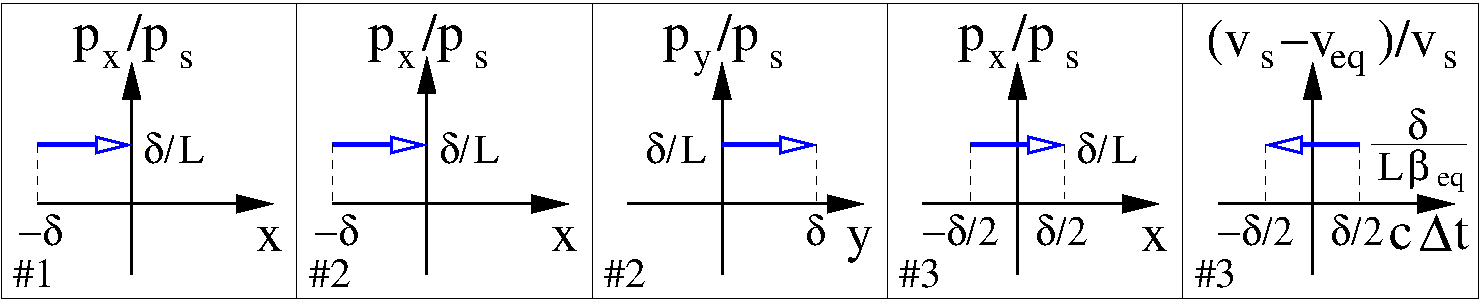
\includegraphics[width=\linewidth]{DriftEx.pdf}
\caption{Schematic draw of phase-space flow in a drift space
		for test particles.}
\label{fig:DriftEx}
\end{figure}
%================================================================================

%--------------------------------------------------------------------------------%
Thus for the drift space of the length $L$ we can write transformation as
\[
\begin{bmatrix}
x			\\ p_x/p_s				\\
y			\\ p_y/p_s				\\
c\,\Delta t \\ (v_s-v_{\text{eq}})/v_s
\end{bmatrix}_{s=L} =
\begin{bmatrix}
1 & L & 0 & 0 & 0 & 0								\\
0 & 1 & 0 & 0 & 0 & 0								\\
0 & 0 & 1 & L & 0 & 0								\\
0 & 0 & 0 & 1 & 0 & 0								\\
0 & 0 & 0 & 0 & 1 & -\frac{L}{\beta_{\text{eq}}}	\\
0 & 0 & 0 & 0 & 0 & 1
\end{bmatrix}
\begin{bmatrix}
x			\\ p_x/p_s				\\
y			\\ p_y/p_s				\\
c\,\Delta t \\ (v_s-v_{\text{eq}})/v_s
\end{bmatrix}_{s=0},
\]
where $c\,\Delta t(s)$ defined as $c(t(s) - t_{\text{eq}}(s))$.
Examples of initial condition for test particles are listed below in
Table~\ref{tab:DriftEx}.
Corresponding phase space flow (except trivial cases) is shown in
Fig.~\ref{fig:DriftEx}.

%================================================================================%
\begin{table}[b!]
\centering
\begin{tabular}{l|c|c|c|c|c|c}
\hline \hline
& \multicolumn{2}{ c| }{Particle \#1}
& \multicolumn{2}{ c| }{Particle \#2}
& \multicolumn{2}{ c  }{Particle \#3}				\\ \cline{2-7}
& ini	& fin	& ini	& fin	& ini	& fin		\\ \hline
$x$							&
	$-q_{\text{off}}$		& 0						&
	$-q_{\text{off}}$		& 0						&
	$-q_{\text{off}}/2$		& $q_{\text{off}}/2$	\\
$p_x/p_s$					&
	$q_{\text{off}}/L$		& $q_{\text{off}}/L$	&
	$q_{\text{off}}/L$		& $q_{\text{off}}/L$	&
	$q_{\text{off}}/L$		& $q_{\text{off}}/L$	\\
$\{p_x/p_{\text{eq}}\}^*$					&
	$\frac{q_{\text{off}}}{L}\frac{p_s}{p_{\text{eq}}}$		&
	$\frac{q_{\text{off}}}{L}\frac{p_s}{p_{\text{eq}}}$		&
	$\frac{q_{\text{off}}}{L}\frac{p_s}{p_{\text{eq}}}$ 	&
	$\frac{q_{\text{off}}}{L}\frac{p_s}{p_{\text{eq}}}$		&
	$\frac{q_{\text{off}}}{L}\frac{p_s}{p_{\text{eq}}}$		&
	$\frac{q_{\text{off}}}{L}\frac{p_s}{p_{\text{eq}}}$		\\
$y$							&
	0						& 0						&
	0						& $q_{\text{off}}$		&
	0						& 0						\\
$p_y/p_s$					&
	0						& 0						&
	$q_{\text{off}}/L$		& $q_{\text{off}}/L$	&
	0						& 0						\\
$\{p_y/p_{\text{eq}}\}^*$					&
	0														&
	0														&
	$\frac{q_{\text{off}}}{L}\frac{p_s}{p_{\text{eq}}}$		&
	$\frac{q_{\text{off}}}{L}\frac{p_s}{p_{\text{eq}}}$		&
	0														&
	0														\\
$c\,\Delta t$ 				&
0							& 0						&
0							& 0						&
$v_{\text{rel}} L/2\,\beta_{\text{eq}}$ & $-v_{\text{rel}} L/2\,\beta_{\text{eq}}$
													\\
$(v_s-v_{\text{eq}})/v_s$	&
0							& 0						&
0							& 0						&
$v_{\text{rel}}$			& $v_{\text{rel}}$		\\
$\{(p-p_{\text{eq}})/p_{\text{eq}}\}^*$	&
0							& 0						&
0							& 0						&
$p_{\text{rel}}$			& $p_{\text{rel}}$		\\
\hline \hline
\end{tabular}
\caption{\label{tab:DriftEx}
		Initial and final sets of coordinates (including the {\it Synergia}'s fixed-z representation, starred variables) for three test particles in drift space, where
		$p_{\text{rel}} + 1 =
		\displaystyle\sqrt{
			\left(\frac{p_x}{p_{\text{eq}}}\right)^2 +
			\left(\frac{p_y}{p_{\text{eq}}}\right)^2 +
			\left(\frac{E  }{E_{\text{eq}}}\right)^2\frac{1}{(1-v_{\text{rel}})^2}
		}$.}
\end{table}
%================================================================================%

\newpage
%================================================================================%
%--------------------------------------------------------------------------------%
%================================================================================%
\subsection{Uniform field (dipole)}

%--------------------------------------------------------------------------------%
The Hamiltonian does not explicitly depend on time-parameter
\begin{subequations}
\begin{align}
	\mathcal{H}[p_x,p_y,p_s;x,y,s;t]\quad\!\! &=
	c \sqrt{ m_0^2c^2 + \mathbf{p}^2 },										\\
	\mathcal{K}[p_x,p_y,-\mathcal{H};x,y,t;s] &=
	- \sqrt{ \left(\frac{\mathcal{H}}{c}\right)^2 - m_0^2c^2 - p_x^2 - p_y^2 }
	- e\,B_0 x,
\end{align}
\end{subequations}

\end{document}